%!TEX root = ./dp5-stability.tex

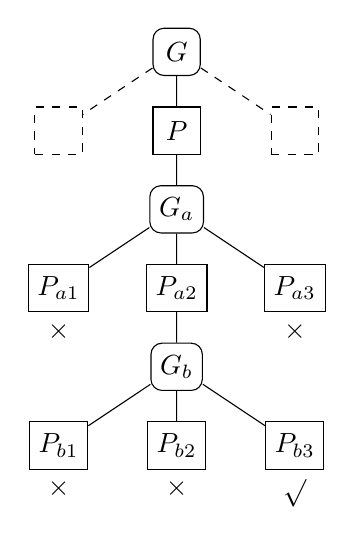
\begin{tikzpicture}[level distance=1.0cm]
\tikzstyle{succ}=[label=below:$\surd$]
\tikzstyle{fail}=[label=below:$\times$]
\tikzstyle{planbox}=[draw,minimum height=0.6cm,minimum width=0.6cm]
\tikzstyle{goalbox}=[draw,rounded corners,minimum height=0.6cm,minimum width=0.6cm]

\node[goalbox] {$G$}
	child[dashed] {node[planbox] {\phantom{$P$}}}
	child[solid] {node[planbox] {$P$}
		child {node[goalbox] (11) {$G_a$}
			child {node[planbox,fail] {$P_{a1}$}}
			child {node[planbox] {$P_{a2}$}
				child {node[goalbox] {$G_{b}$}
					child {node[planbox,fail] {$P_{b1}$}}
					child {node[planbox,fail] {$P_{b2}$}}
					child {node[planbox,succ] {$P_{b3}$}}
				}
			}
			child {node[planbox,fail] {$P_{a3}$}}
		}
	}
	child[dashed] {node[planbox] {\phantom{$P$}}}
;
\end{tikzpicture}


